%----------------------------------------------------------------------------
\chapter{\caseStudy}
%----------------------------------------------------------------------------

\section{A tanulmány háttere}
Az esettanulmány során egy kitalált, de mégis valósághű vasúti fékrendszert tervezek és elemzem biztonsági szempontból.
A rendszert a lentebb (lásd: \ref{requirements}. fejezet) részletezett követelmények alapján, továbbá az itt említett működési körülményeknek megfelelően tervezem.

A vasútipart és ezzel együtt a vasútifék-technológiát az utóbbi időben rohamos fejlődés határozta meg. 
Számos működési elv elérhető az iparágban (pneumatikus, hidraulikus, elektro-pneumatikus, elektro-hidraulikus, elektromágneses), amelyeknek mind meg van a maga előnye és hátránya.

Ebben a dolgozatban egy összetett integrált fékrendszer megoldást szeretnék modellezni, mely rendelkezik egy fékvezérlő berendezéssel.
Ezért az elavultnak számító és mára leginkább csak a vasúti teherszállításban - az egyszerűsége és költséghatékonysága miatt - használt pneumatikus és a szintén tisztán fizikai elven működő hidraulikus rendszereket nem találtam alkalmasnak a dolgozat témájához.

Napjainkban fontos téma, többek között a globális felmelegedés és a ${CO}_2$ kibocsátás visszaszorítása - melyek részletei és elemzése nem képezik ennek a dolgozatnak részét - miatt, a tömegközlekedés.
A vasútipar emberek szállítmányozására alkamas része is több alrészre bontható, nagysebességű(>300 km/h)/intercity vonatok, 
regionális/ingázó vonatok (pl: Budapesti HÉV), metró, könnyű vasúti vonatok/villamosok.

A dolgozat során egy modern alacsonypadlós városi tömegközlekedésre alkalmas villamos rendszerén keresztül szeretném bemutatni a modell alapú rendszertervezés (Model-based Systems Design, MBSD) módszertanait és az elkészült rendszer biztonsági és megbízhatósági analízisét. 
Mivel az alacsonypadlós villamosokon véges hely áll rendelkezésre, ezért egy kompakt megoldásra van szükség. 
Továbbá, biztosítani kell bármely közlekedési helyzetben a szerelvény biztonságos és optimális lassulását, megállását.

A rendszer működési körülményeit leginkább az Európai kontinensen lévő időjárási és hőmérsékleti viszonyoknak megfelelően tervezem és megfelelő biztonsági és megbízhatósági kalkulációkat is ennek megfelelően készítem.

\section{Követelmények} \label{requirements}
\begin{figure}
    \centering
    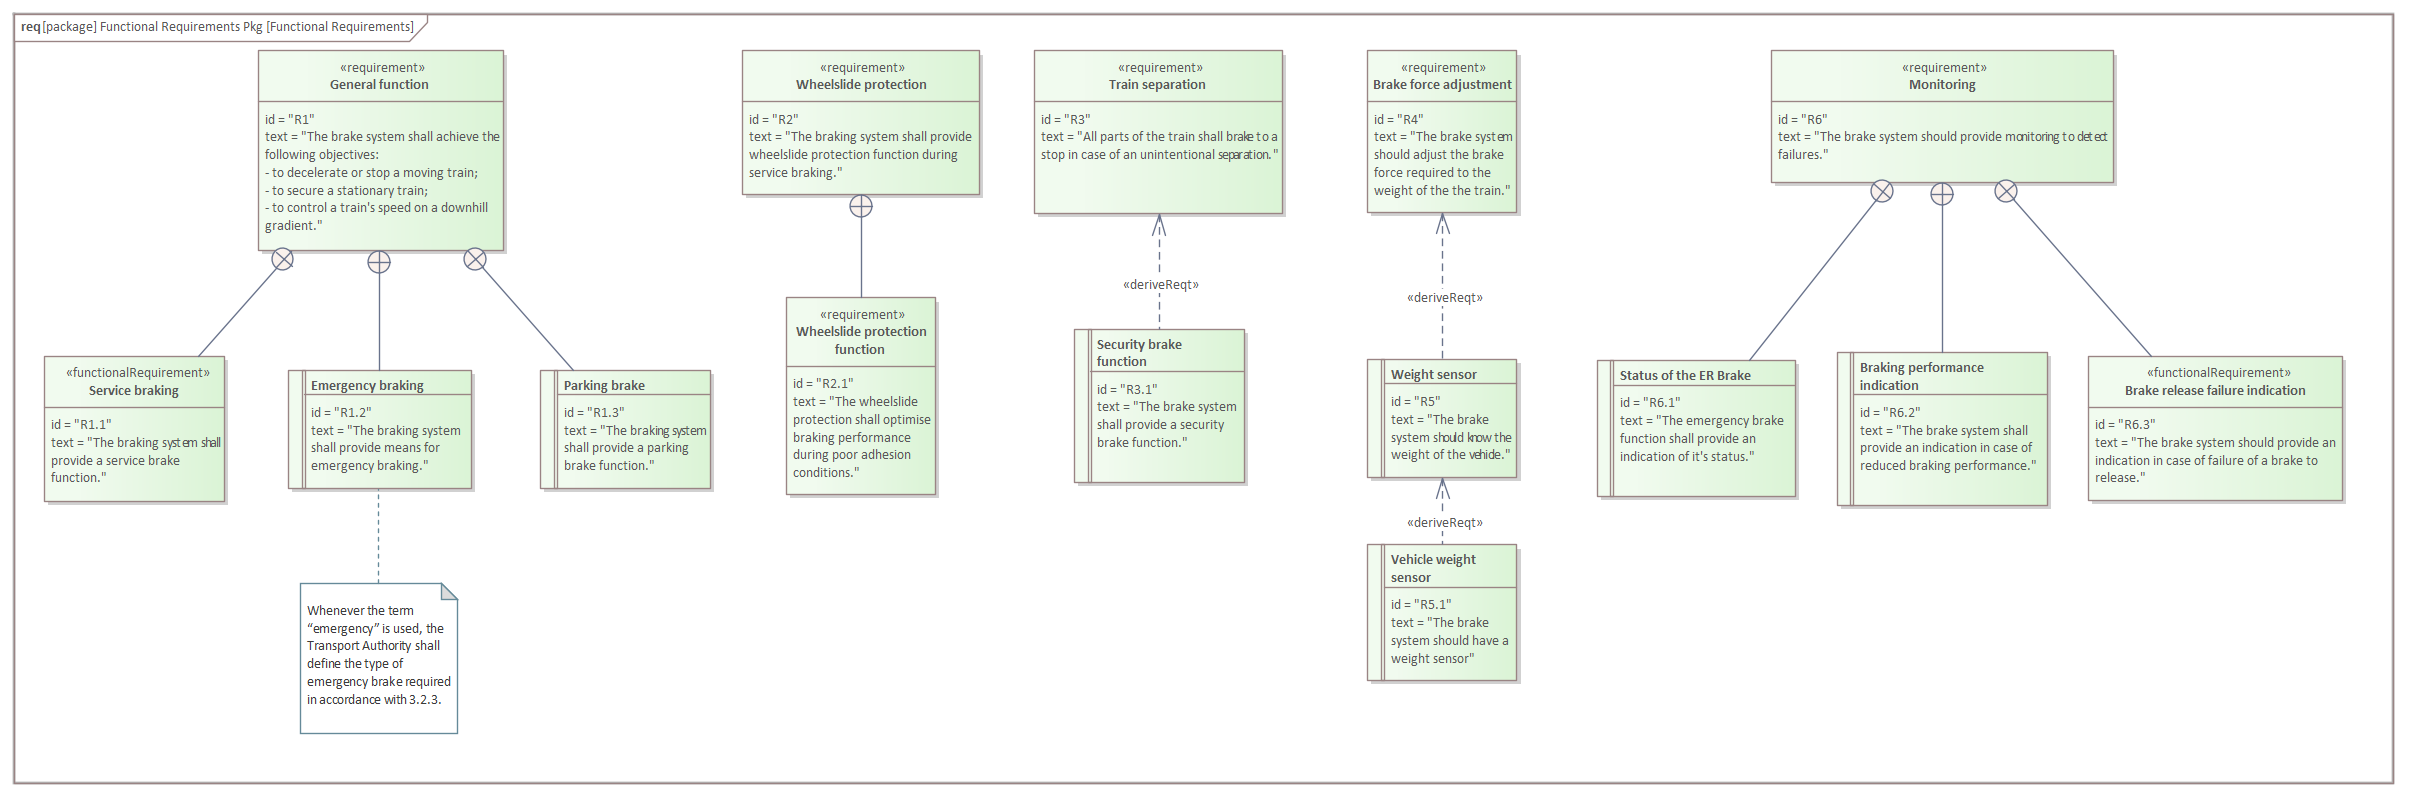
\includegraphics[width=150mm, keepaspectratio]{figures/Functional Requirements.png}
    \caption{Functionális követelmények}
    \label{fig:FunReq}
\end{figure}